\documentclass[CS5104-Notes.tex]{subfiles}
\begin{document}

\section{Linear regression}
Linear regression models are simple but can provide a good and adequate descriptions of how the inputs affect the output. As linear regression only deals with linear models, it follows from the linear line equation $y = mx + c$ where the gradient $m$ and intercept $c$ are the $\theta$ parameters that the model tries to learn. This can be rewritten as:
\begin{equation}
f(X, \theta) = \theta_{0} + \theta_{1}X_{1}
\end{equation}
where $\theta_{0}$ represents the $c$ intercept and $\theta_{1}$ represents the $m$ gradient.
\n
Furthermore, a loss function has to be defined to evaluate the quality of the fit without manual inspection. The goal of training is to reduce the error of the loss function. This is done by trying lots of different $\theta$ values and computing the error each time. 

\subsection{Gradient descent}
Gradient descent is a method for parameter optimisation which automatically gets to the best model by minimising the lost function and automatically altering the $\theta$ parameters.
\begin{equation}
  \theta_{j} := \theta_{j} - \alpha \frac{\delta}{\delta \theta_{j}} L(\theta_{0}, /theta_{1})
\end{equation}
where j = 0 and j = 1 update is done simultaneously. $\alpha$ here is the learning rate, which acts as a modifier to how much should be updated on each iteration. $\frac{\delta}{\delta \theta_{j}} L(\theta_{0}, /theta_{1})$ is the derivative. The derivative of the loss function is used to see if we should increase or decrease the value of $\theta$.
\begin{figure}
  \centering
  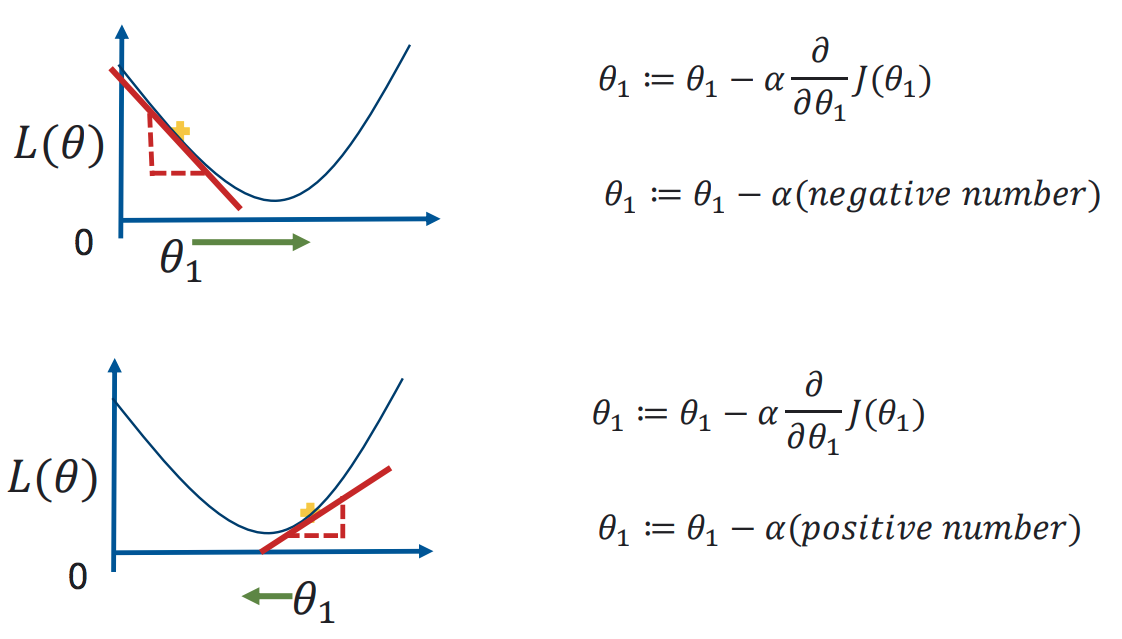
\includegraphics[width=0.9\textwidth, keepaspectratio]{imgs/gradient-descent.png}
  \caption{Gradient descent updating based on positive or negative gradient. For example, if the gradient is negative, we want to increase the $\theta$ values and recalculate the gradient.}
\end{figure}
There is an issue with gradient descent where it can get stuck in an local minimumm rather than the global minimum. There are a few ways of dealing with this:
\begin{itemize}
\item Try different initial values to start at different locations in the search space
\item Add momentum to roll over local minima
\end{itemize}

\subsection{Multivariate linear regression}
Linear models can have many features and by extending to $n$ features with $n$ $\theta$ parameters. This extends the linear equation to be:
\begin{equation}
f(x) = \theta_{0} + \theta_{1}x_{1} + \theta_{2}x_{2} + ... \theta_{n}x_{n}
\end{equation}
The input features $X$ and parameters $\theta$ can be more easily represented with matrix form:
\begin{equation}
X = \begin{bmatrix}
X_{0} \\
X_{1} \\
X_{2} \\
\vdots \\
X_{n}
\end{bmatrix}
\end{equation}
Using matrix operations, all $\theta$ parameters can be updated simultaneously on every step rather than separately.

\subsection{Feature scaling}
When there are many input features, they can come from different scales. For example, one feature may have the range 0-1 while another has values ranging from 100-1000. Because of these different scales, the larger values may dominate the model even if both features are equally important. To deal with this issues, all features can be scaled to the same range through normalisation.

\end{document}